%*********************************************************************
%	APPENDIX: SYSTEM WIRING
%*********************************************************************
%*********************************************************************
%   APPENDIX: PT1000 ICE BATH CHECK
%   Belongs to Chapter 5, Commissioning and Instrumentation.
%   Referenced from Section 5.4.1 as app:icebath.
%   Small enough to be pasted into appendix_wiring.tex as a second
%   section if you would rather not have another appendix letter.
%*********************************************************************
\chapter{Commissioning and Instrumentation}
\label{app:commissioning}

This appendix supports Chapters~\ref{ch:commissioning} to~\ref{ch:ClosedLoop}. It shows the printed enclosure, gives the full PT1000 ice bath check, and lists the wiring of the prototype and the test setup used for the thermal tests.

\section{Printed Enclosure}
\label{app:printed-enclosure}

Figure~\ref{fig:enclosure-built} shows the printed enclosure assembled, with a 96-well plate under the ITO glass lid and the cable gland and gas fitting in the end wall. Figure~\ref{fig:enclosure-stage} shows it sitting in the K-frame insert of the microscope stage it was designed for (Section~\ref{sec:build-observations}).

\begin{figure}[H]
    \centering
    \begin{subfigure}[b]{0.4\textwidth}
        \centering
        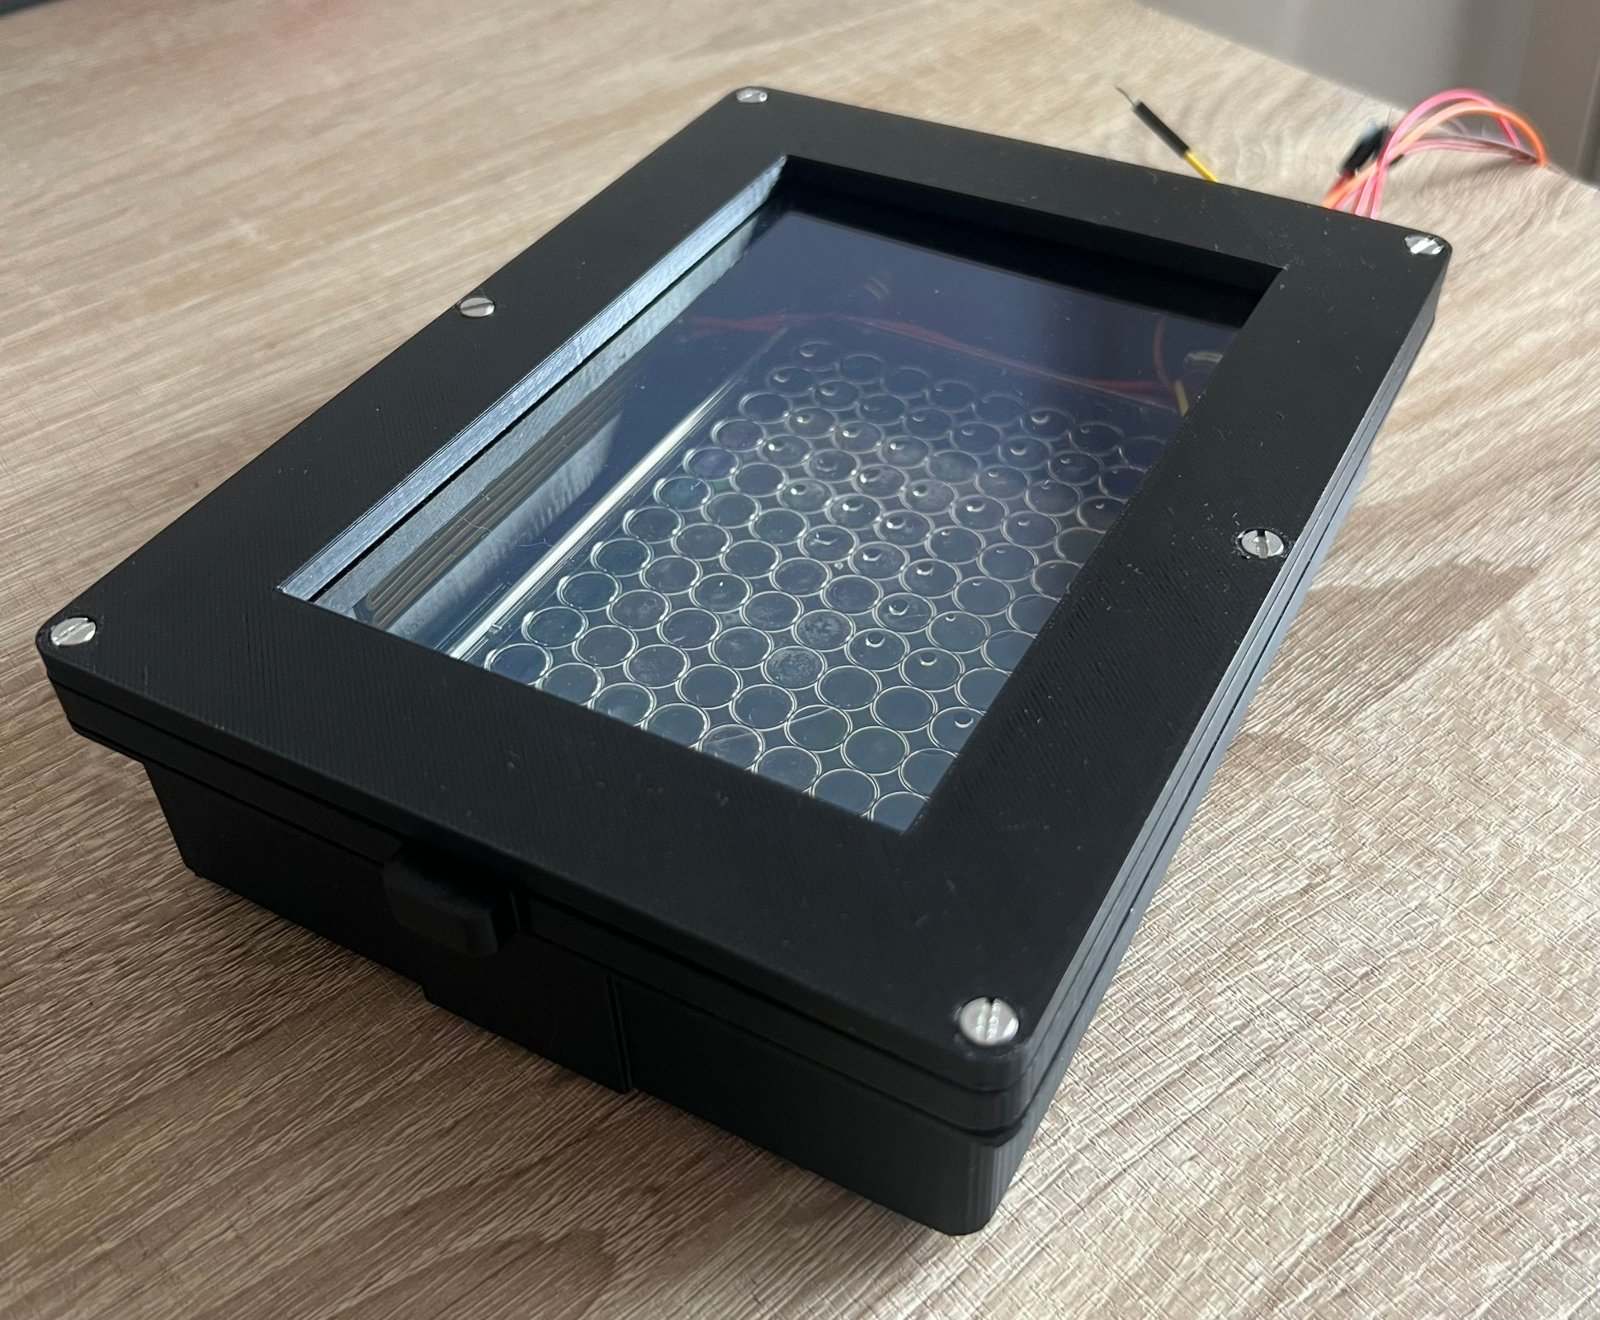
\includegraphics[width=\linewidth]{figs/ch5/enclosure_printed_top.jpg}
        \caption{}
        \label{fig:enclosure-top}
    \end{subfigure}\hfill
    \begin{subfigure}[b]{0.4\textwidth}
        \centering
        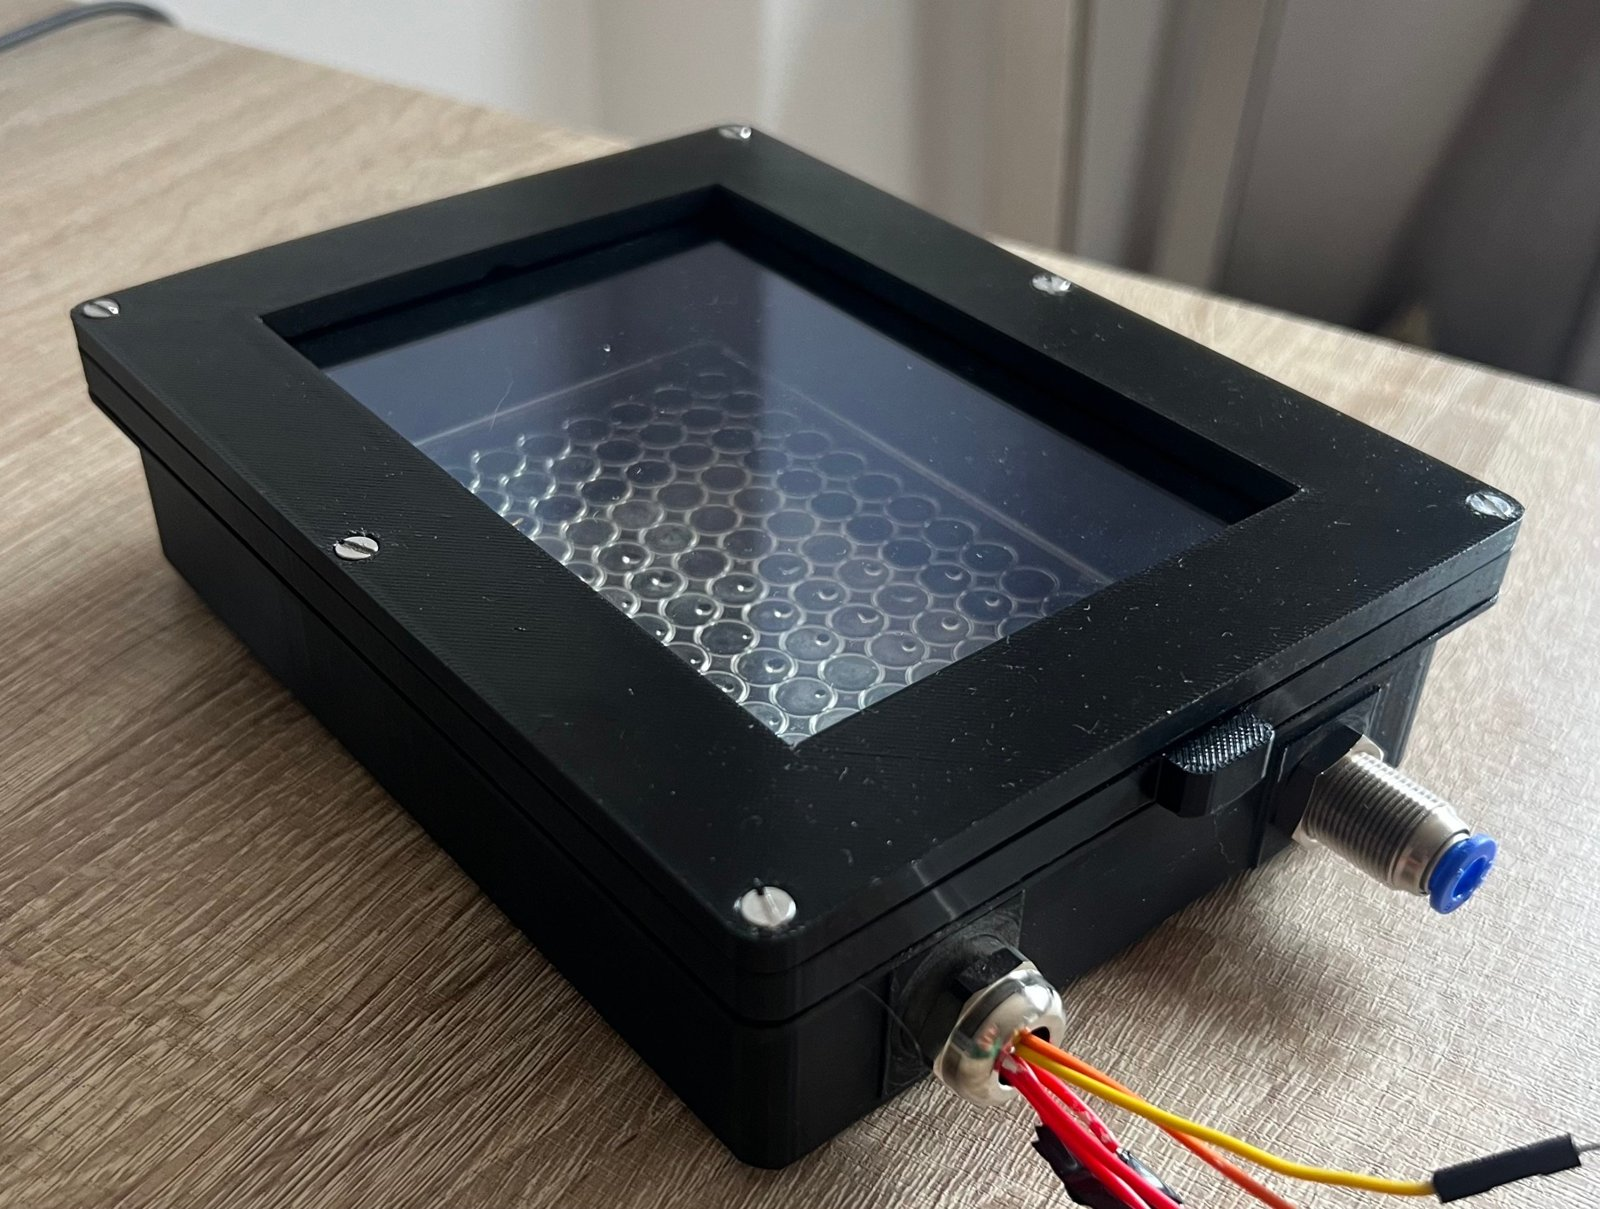
\includegraphics[width=\linewidth]{figs/ch5/enclosure_printed_fittings.jpg}
        \caption{}
        \label{fig:enclosure-fittings}
    \end{subfigure}
    \caption[The printed enclosure as built]{\textbf{The printed enclosure as built.} (a) Assembled, with the plate under the ITO glass lid. (b) The end wall, with the cable gland for the wires and the push-in fitting for the gas line.}
    \label{fig:enclosure-built}
\end{figure}

\begin{figure}[H]
    \centering
    \begin{subfigure}[b]{0.50\textwidth}
        \centering
        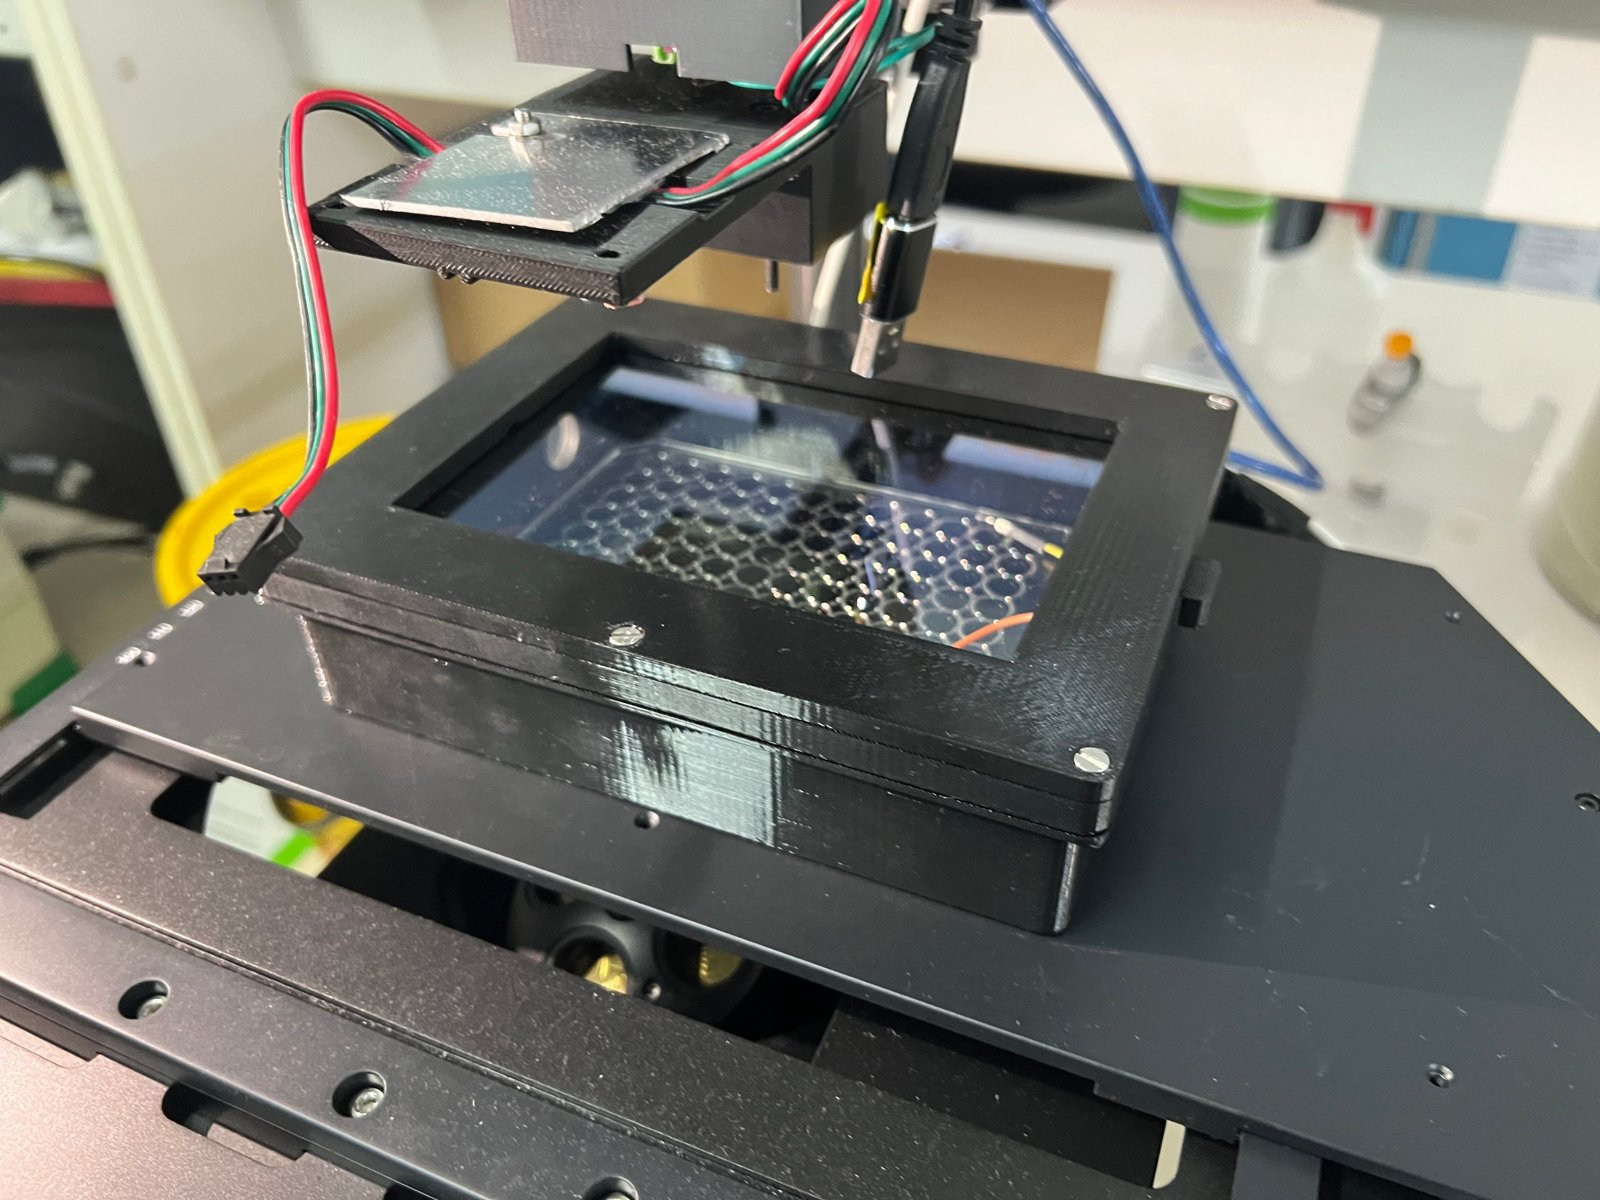
\includegraphics[width=\linewidth]{figs/ch5/enclosure_on_stage_side.jpg}
        \caption{}
        \label{fig:enclosure-stage-side}
    \end{subfigure}\hfill
    \begin{subfigure}[b]{0.36\textwidth}
        \centering
        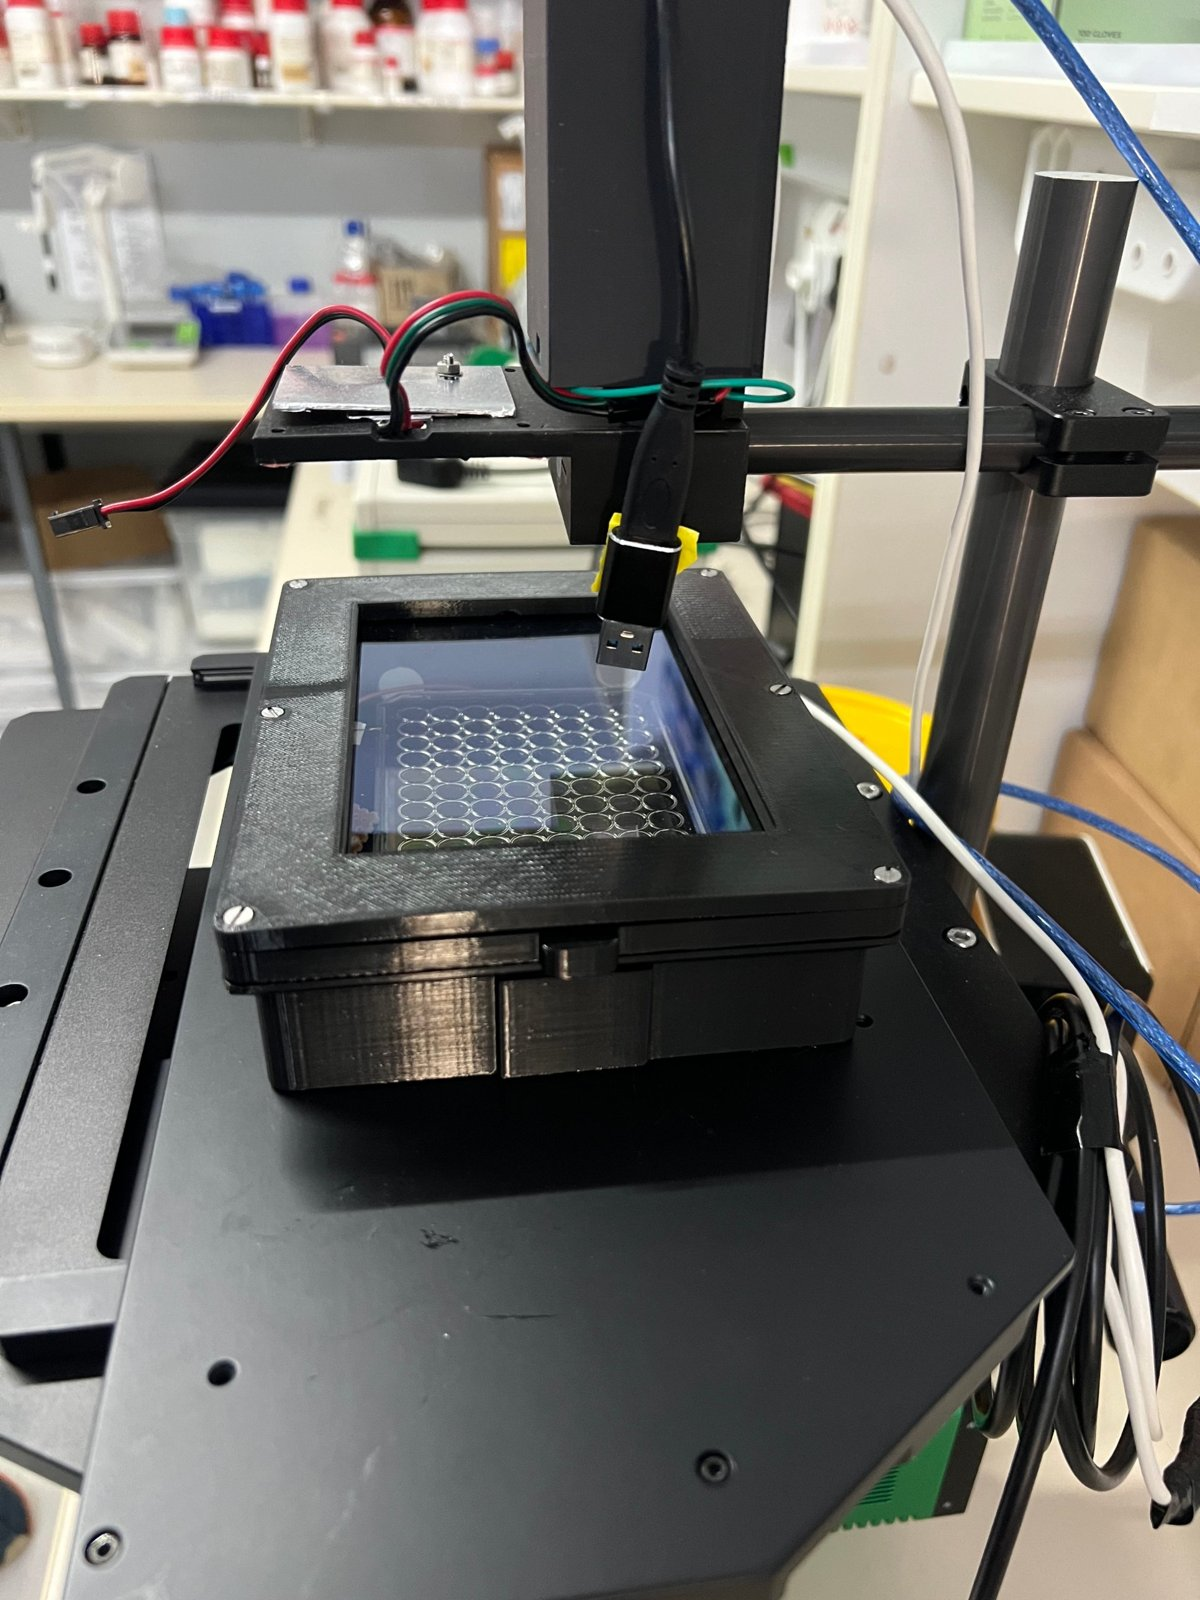
\includegraphics[width=\linewidth]{figs/ch5/enclosure_on_stage_front.jpg}
        \caption{}
        \label{fig:enclosure-stage-front}
    \end{subfigure}
    \caption[The enclosure fitted to the microscope stage]{\textbf{The enclosure fitted to the microscope stage.} (a) Side view, with the base sitting flat in the K-frame insert. (b) Front view, with the plate centred over the stage opening.}
    \label{fig:enclosure-stage}
\end{figure}

\FloatBarrier

\section{PT1000 Ice Bath Check}
\label{app:icebath}

The PT1000 was checked against an ice bath twice. The first bath was made quickly and the second carefully, so that an error in the ice could be told apart from an error in the measurement. Figure~\ref{fig:ch5-icebath} shows both runs.

The first bath used ice cubes and a little cold water, and settled at 1001.15\,$\Omega$, or $+0.29$\,\textdegree{}C, over the last minute of a four-minute run. For the second bath, the ice was crushed in a blender, drained, and packed tightly into an insulated container with just enough cold water to fill the gaps. The probe was pushed in well past its tip and kept away from the sides and bottom. This bath settled at 1001.02\,$\Omega$, or $+0.26$\,\textdegree{}C, over its last 100\,s, with a standard deviation of 0.023\,\textdegree{}C. The two baths agree to within 0.03\,\textdegree{}C, which is less than one converter step (0.034\,\textdegree{}C). Since a quick bath and a careful bath gave the same result, the ice did not cause the offset. The extra 1.02\,$\Omega$ is the resistance of the 2-wire leads and their connections.

\begin{figure}[htbp]
    \centering
    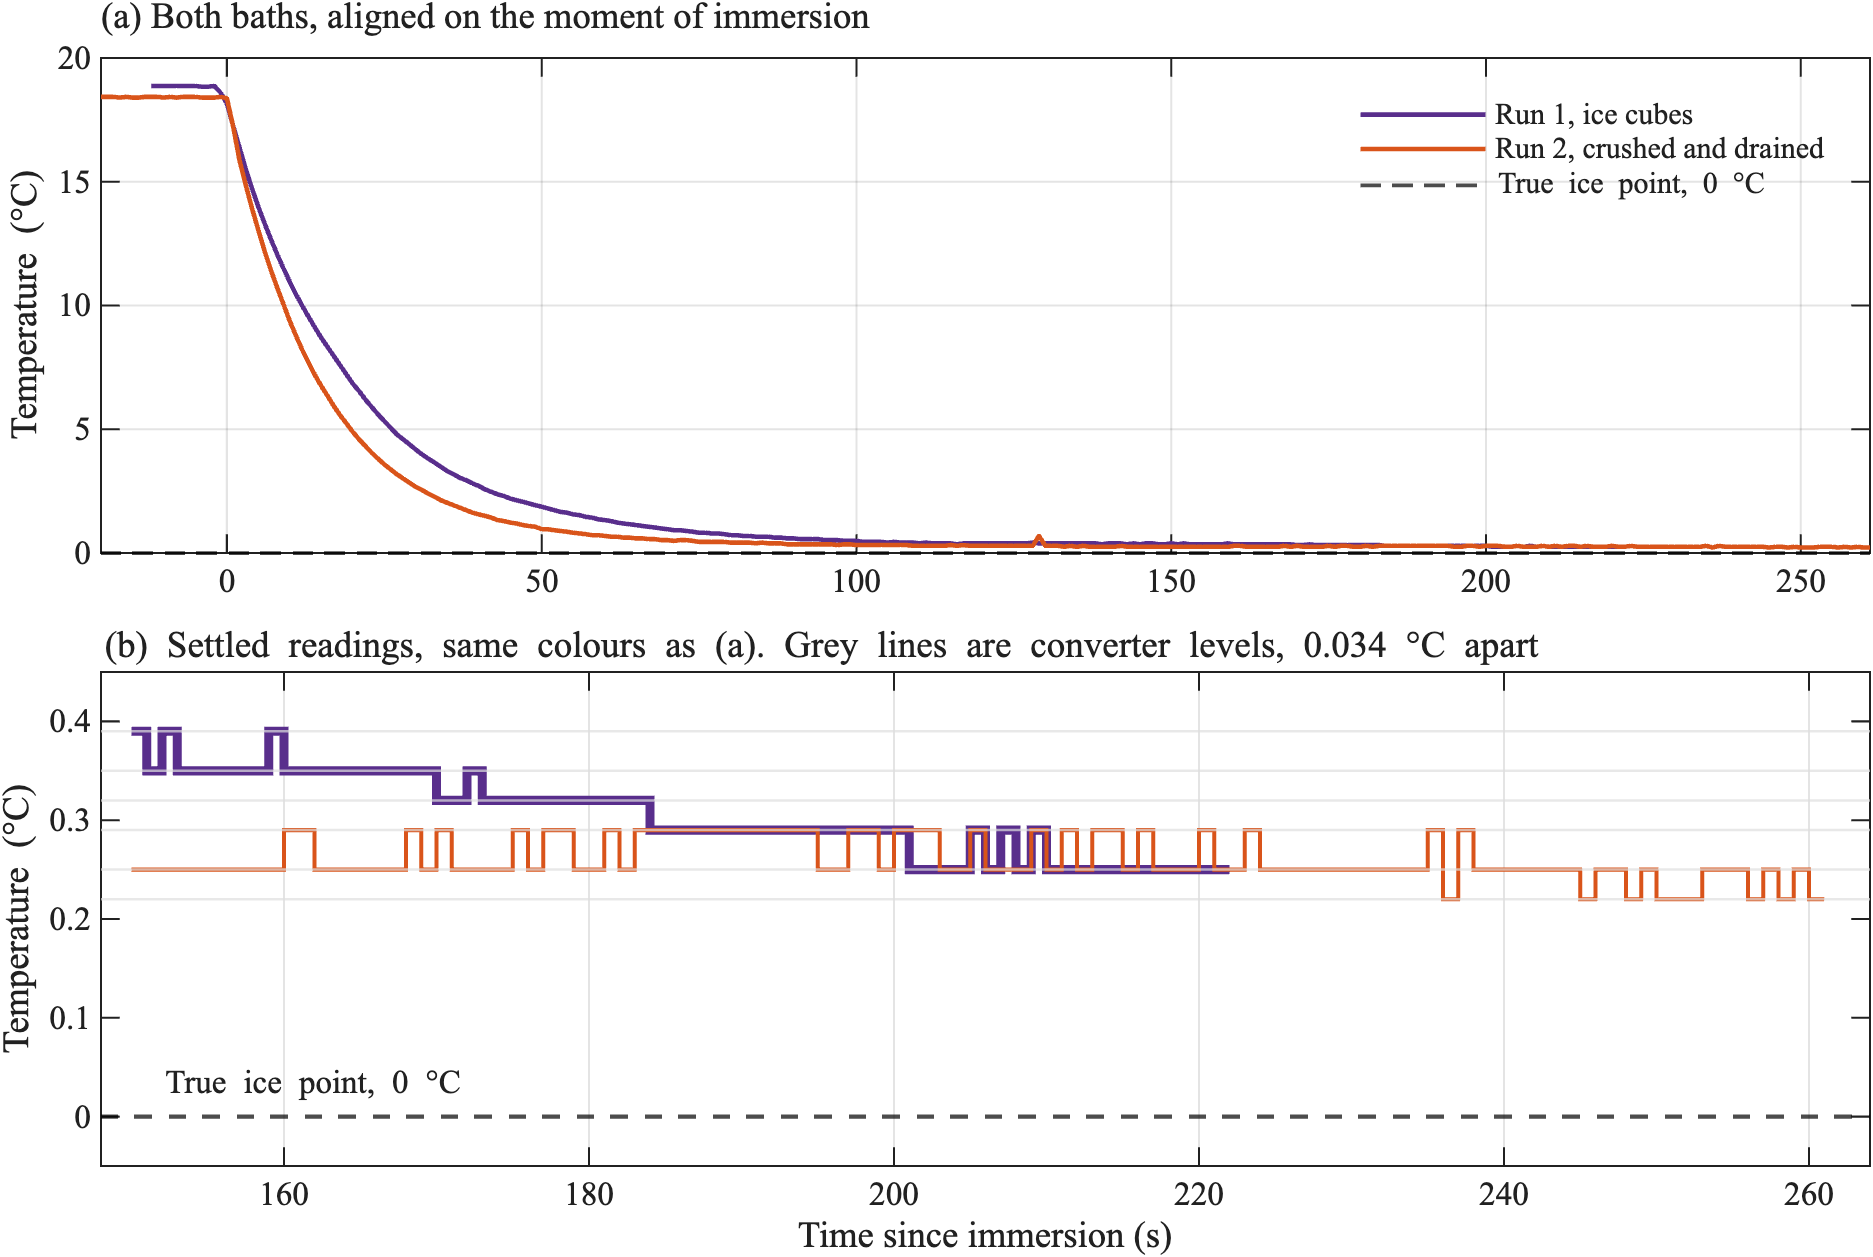
\includegraphics[width=0.65\textwidth]{figs/ch5/fig_M2_pt1000_icebath.png}
    \caption[PT1000 ice bath check]{\textbf{PT1000 ice bath check with two separately made baths.} (a) Both runs, timed from when the probe went in. Run 1 used ice cubes and run 2 used crushed, drained ice. (b) The settled end of each run, with the levels the converter can read shown in grey. The two averages differ by less than one level, so the offset comes from the measurement and not the ice.}
    \label{fig:ch5-icebath}
\end{figure}


\FloatBarrier
\section{System Wiring}
\label{app:wiring}

This section lists every electrical connection in the prototype, so that it can be rebuilt. Module pins are named as they are labelled on each board, and Nucleo pins are given by their Arduino header name with the STM32 pin in brackets. The heater driver and the thermistor dividers are drawn in Figure~\ref{fig:driver-circuits}. Table~\ref{tab:wiring} lists all the connections, including the BMP280 and DHT22 that were added for the long run in Section~\ref{sec:humidity}.

The table shows the wall heater on D4. The glass heater and the heated base in Chapter~\ref{ch:ClosedLoop} use the same driver circuit on other PWM pins, avoiding D8 and D2 (used by the ExplorIR-M) and D10 to D15 (used by the two converters).
% TODO (Lauren): add the glass and base heater pins as rows in the table below.
Each thermistor's fixed resistor was measured instead of using its nominal value, because a 1\% resistor error alone gives about $\pm$0.2\,\textdegree{}C, as much as the thermistor's own tolerance.

{\scriptsize
\setlength{\tabcolsep}{5pt}
\renewcommand{\arraystretch}{1.12}
\begin{longtable}{@{}>{\raggedright\arraybackslash}p{3.1cm}>{\raggedright\arraybackslash}p{3.9cm}>{\raggedright\arraybackslash}p{7.0cm}@{}}
\caption[System connection table]{\textbf{System connection table.} Every pin on every module and what it connects to, including unused pins.} \label{tab:wiring} \\
\toprule
        \textbf{Pin} & \textbf{Connects to} & \textbf{Function} \\
        \midrule
\endfirsthead
\multicolumn{3}{@{}l}{\footnotesize\textit{Table~\ref{tab:wiring} continued}} \\
\toprule
        \textbf{Pin} & \textbf{Connects to} & \textbf{Function} \\
        \midrule
\endhead
\bottomrule
\endlastfoot

        \addlinespace[1pt]
        \multicolumn{3}{@{}l}{\textit{MAX31865 RTD converter, SPI}} \\
        \addlinespace[2pt]
        3V3 & Nucleo 3V3 & Supply. On-board regulator removed, see Section~\ref{subsec:pt1000-commissioning} \\
        VIN & Nucleo 3V3 & Tied to 3V3 so level shifting shares one rail \\
        GND & Nucleo GND & \\
        CLK & D13 (PA5) & SPI clock \\
        SDO & D12 (PA6) & Data out of the converter, into the Nucleo \\
        SDI & D11 (PA7) & Data into the converter \\
        CS  & D10 (PB6) & Chip select \\
        F+, F$-$ & PT1000 leads & 2-wire mode, both wire-select jumpers soldered closed \\
        RDY & not connected & Code polls instead \\
        \addlinespace[4pt]
        \midrule
        \addlinespace[1pt]
        \multicolumn{3}{@{}l}{\textit{ADS1115 thermistor converter, I\textsuperscript{2}C}} \\
        \addlinespace[2pt]
        VDD & Nucleo 3V3 & Measured 3.29\,V, used in the conversion \\
        GND & Nucleo GND & \\
        SCL & D15 (PB8) & Shared bus with the SCD30 \\
        SDA & D14 (PB9) & Shared bus with the SCD30 \\
        ADDR & GND & Sets address 0x48 \\
        A0 & T1 divider & Fixed resistor 9.84\,k$\Omega$ (Figure~\ref{fig:driver-circuits}b) \\
        A1 & T2 divider & Fixed resistor 9.98\,k$\Omega$ \\
        A2 & T3 divider & Fixed resistor 9.89\,k$\Omega$ \\
        A3 & T4 divider & Fixed resistor 9.94\,k$\Omega$ \\
        \addlinespace[4pt]
        \midrule
        \addlinespace[1pt]
        \multicolumn{3}{@{}l}{\textit{SCD30 CO\textsubscript{2}, temperature and humidity, I\textsuperscript{2}C}} \\
        \addlinespace[2pt]
        1 VDD & Nucleo 3V3 & \\
        2 GND & Nucleo GND & \\
        3 TX/SCL & D15 (PB8) & Shared bus with the ADS1115 \\
        4 RX/SDA & D14 (PB9) & Shared bus with the ADS1115 \\
        5 RDY & not connected & \\
        6 PWM & not connected & \\
        7 SEL & not connected & Floating selects I\textsuperscript{2}C \\
        \addlinespace[4pt]
        \midrule
        \addlinespace[1pt]
        \multicolumn{3}{@{}l}{\textit{BMP280 room temperature, I\textsuperscript{2}C (long run only)}} \\
        \addlinespace[2pt]
        VCC & Nucleo 3V3 & 3.3\,V module \\
        GND & Nucleo GND & \\
        SCL & D15 (PB8) & Shared bus with the ADS1115 \\
        SDA & D14 (PB9) & Shared bus with the ADS1115 \\
        SDO & GND & Sets address 0x76 \\
        \addlinespace[4pt]
        \midrule
        \addlinespace[1pt]
        \multicolumn{3}{@{}l}{\textit{DHT22 humidity and temperature, single-wire (long run only)}} \\
        \addlinespace[2pt]
        VCC & Nucleo 3V3 & \\
        DATA & A5 (PC0) & Single-wire bus, internal pull-up enabled \\
        GND & Nucleo GND & \\
        \addlinespace[4pt]
        \midrule
        \addlinespace[1pt]
        \multicolumn{3}{@{}l}{\textit{ExplorIR-M-E-100 CO\textsubscript{2} sensor, UART}} \\
        \addlinespace[2pt]
        1 Rx\_In & D8 (PA9) & Commands into the sensor \\
        2 Tx\_Out & D2 (PA10) & Readings out of the sensor \\
        3 0V & Nucleo GND & \\
        4 V+ & Nucleo 3V3 & \\
        \addlinespace[4pt]
        \midrule
        \addlinespace[1pt]
        \multicolumn{3}{@{}l}{\textit{Relay module, CO\textsubscript{2} solenoid}} \\
        \addlinespace[2pt]
        VCC & Nucleo 5V & \\
        GND & Nucleo GND & \\
        IN & D7 (PA8) & Open-drain, active low, see Section~\ref{sec:power-commissioning} \\
        COM & Solenoid side of the cut brown conductor & \\
        NO & Plug side of the cut brown conductor & Mains on NO so no terminal is live when off \\
        NC & not connected & \\
        \addlinespace[4pt]
        \midrule
        \addlinespace[1pt]
        \multicolumn{3}{@{}l}{\textit{Heater driver, one channel per heated zone}} \\
        \addlinespace[2pt]
        PN2222A base & Nucleo PWM pin through 150\,$\Omega$ & Wall heater channel on D4 \\
        PN2222A base & GND through 10\,k$\Omega$ & Holds the heater off while the STM32 boots \\
        PN2222A emitter & TIP31C base & Darlington pair \\
        PN2222A collector & TIP31C collector & \\
        TIP31C base & GND through 1\,k$\Omega$ & Clean turn-off \\
        TIP31C collector & Heater low side & \\
        TIP31C emitter & GND & Common ground with the 12\,V supply \\
        Heater high side & $+12$\,V rail & \\
        \addlinespace[4pt]
        \midrule
        \addlinespace[1pt]
        \multicolumn{3}{@{}l}{\textit{Power}} \\
        \addlinespace[2pt]
        AC-DC adapter out & $+12$\,V rail & Measured 12.44\,V \\
        Buck converter in & $+12$\,V rail & \\
        Buck converter out & 5\,V rail & Set and confirmed at 5\,V \\
        Supply GND & Nucleo GND & Single common ground for the whole system \\
        Mains & Relay and solenoid only & Kept in a closed enclosure, see Section~\ref{sec:power-commissioning} \\
        
    \end{longtable}
}

%*********************************************************************
% End of System Wiring
%*********************************************************************